\documentclass[12pt, a4paper]{article}

\usepackage{amsmath,amsfonts,amssymb,amsthm,mathtools}

\usepackage{fontspec}         % пакет для подгрузки шрифтов
\setmainfont{Georgia}          % задаёт основной шрифт документа

\usepackage{unicode-math}     % пакет для установки математического шрифта
\setmathfont{Asana Math}      % шрифт для математики

\usepackage{graphicx}

\usepackage{polyglossia}      % Пакет, который позволяет подгружать русские буквы
\setdefaultlanguage{russian}  % Основной язык документа
\setotherlanguage{english}    % Второстепенный язык документа

%% Неравенства с косыми чёртачками
\renewcommand{\le}{\leqslant}
\renewcommand{\ge}{\geqslant}

\begin{document}

\section{10 фактов о себе}

\begin{enumerate}
\item Я не люблю рассказывать о себе просто так
\item Поэтому в этом задании я ограничусь очевидными фактами
\item Меня зовут Аня
\item Мне 19
\item Я учусь в РАНХиГС
\item На отделении экономики
\item И каждый день строю планы побега
\item А потом передумываю
\item Раньше я верила, что люблю математику
\item Сейчас поняла, что люблю здоровый сон и отдых 
\end{enumerate}

\section{Фото}
У меня на компьютере нет моих фотографий. Зато у меня есть фотография моего котика!

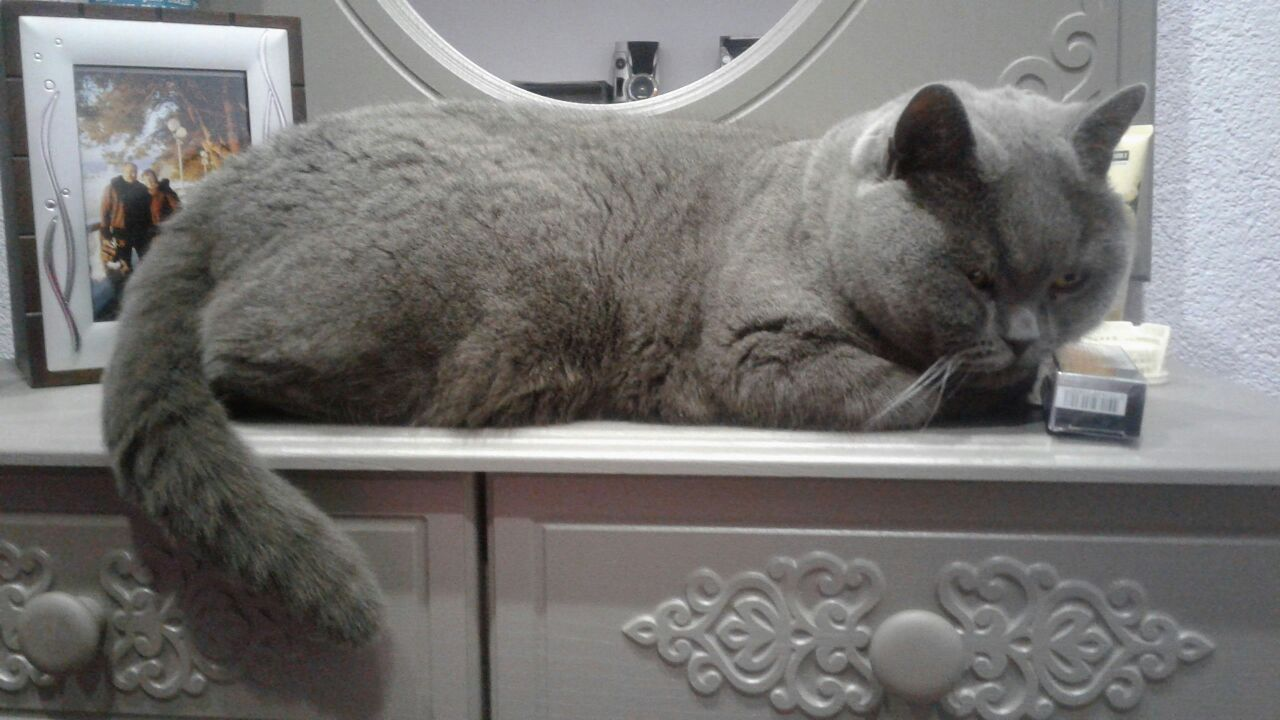
\includegraphics[scale=0.25]{cat.jpg}

\section{5 любимых формул +1}

\begin{equation} \label{n1}
\exists \text{(конечный)} \lim_{n \to \infty} x_n  \Leftrightarrow \forall \varepsilon > 0 \quad  \exists N(\varepsilon) : \forall n, m > N(\varepsilon) \quad |x_n - x_m| < \varepsilon 
\end{equation}

\begin{equation} \label{n2}
\sum_{n=1}^{\infty} a_n \quad \text{сходится}  \Leftrightarrow  \forall \varepsilon > 0 \quad  \exists N(\varepsilon) : \forall n \ge m > N(\varepsilon) \quad |a_{m+1}+a_{m+2}+...+a_n|< \varepsilon 
\end{equation}

\begin{equation} \label{n3}
q = \lim_{n \to \infty} \frac{a_{n+1}}{a_n} 
\end{equation}

\begin{enumerate}
\item q<1 - ряд сходится абсолютно
\item q>1 - ряд расходится
\item q=1 - неизвестно, сходится ряд или расходится
\end{enumerate}

\begin{multline} \label{n4}
	 (x + y)^5 = (x+y)\cdot(x+y)\cdot(x+y)\cdot(x+y)\cdot(x+y) = \\
	 = x^5 + 5x^4y + 10x^3y^2 + 10x^2y^3 + 5xy^4 + y^5 
\end{multline}

\begin{equation} \label{n5}
 \int sh x dx = ch x + C 
\end{equation}

\begin{equation} \label{n6}
H(f) =
 \begin{bmatrix}
   \frac{\partial^2f}{\partial x_1^2} & \frac{\partial^2f}{\partial x_1 \partial x_2} & \cdots &  \frac{\partial^2f}{\partial x_1\partial x_n}  \\
  \frac{\partial^2f}{\partial x_2\partial x_1} & \frac{\partial^2f}{\partial x_2^2} & \cdots & \frac{\partial^2f}{\partial x_2\partial x_n}  \\
  \vdots  & \vdots  & \ddots & \vdots  \\
 \frac{\partial^2f}{\partial x_n\partial x_1}  & \frac{\partial^2f}{\partial x_n\partial x_2}  & \cdots & \frac{\partial^2f}{\partial x_n^2}
 \end{bmatrix}
\end{equation}


Я люблю признак сходимоти числовой последовательности Коши - уравнение \ref{n1}, потому что это начало начал! Это самая первая формула Коши, которую мы выучили в матане, и я помню, какой ужас она тогда вызывала. Я люблю признак Даламбера (\ref{n3}), потому что Артем Иванович много пар подряд смеялся над тем, что мы "Даламберовская группа" и весь семестр проходим только этот признак. Ну и пусть, зато теперь мы навсегда запомним хоть одну формулу матанализа. Я люблю эту непонятную штуку из таблицы интегрироваия - уравнение \ref{n5}, потому что я проучилась уже 3 семестра на отделении, где "ой, у нас так много математики", и до сих пор понятия не имею, что это за ерунада, и вряд ли когда-нибудь этим воспользуюсь.


\end{document}





